\documentclass[10pt]{article}


%%
% slight detour to create the proper text/paper size.
% Depends on the ifthen package, needed before loading
% the geometry package
%%

\usepackage{ifthen}
\newboolean{tabletsize}
\setboolean{tabletsize}{false}

\usepackage{lipsum}
\usepackage{pgfplots}
\pgfplotsset{compat=1.13}
\pgfplotsset{colormap={coloronemap}{rgb=(.4,.4,1); rgb=(.8,.8,1)}}
\pgfplotsset{colormap={colortwomap}{rgb=(1,.4,.4); rgb=(1,.8,.8)}}
%\pgfplotsset{compat=1.3}
\usepackage{eso-pic,calc}
\usepackage[font=small]{caption}
\usepgfplotslibrary{external}
\usetikzlibrary{calc}
\usetikzlibrary{shadings}

\usepackage[h]{esvect}

	%\newcounter{chapter}
	%\newcommand{\chapter}{\refstepcounter{chapter}\Huge Chapter \thechapter \vskip 2\baselineskip\normalsize}
%%%%%%\tikzexternalize[prefix=figures/]


%


%\pgfplotsset{width=\marginparwidth+1pt,compat=1.3}
%\pgfplotsset{compat=1.8}

%
%	Note how the tablet version differs from the booksize only in 
% the size of the margins.
%
% Changing the following isn't hard but should be done with 
% practice and care, making sure to get the margins right for a 
% particular page size and printing format
%
%% Layout for printed book through Amazon CreateSpace, perfect bound,
%% 8.5 x 11 paper size, 1in inner margin, 1/2in (roughly) outer margin
%\newboolean{longpage}
%\setboolean{longpage}{false}

%\ifthenelse{\boolean{tabletsize}}{\usepackage[paperheight=11in,paperwidth=8.5in, inner=1in,includeheadfoot,textheight=9in,textwidth=345pt,marginparwidth=150pt]{geometry}
%}{\usepackage[paperheight=11in,paperwidth=8.5in, inner=1in,includeheadfoot,textheight=9in,textwidth=345pt,marginparwidth=150pt]{geometry}
%}

\usepackage[paperheight=11in,paperwidth=3in,%inner=1in,includeheadfoot,
textheight=10in,%textwidth=345pt,
marginparwidth=150pt]{geometry}
%% end detour
%%
\usepackage{amsmath}
\usepackage{pifont}
%\usepackage{APEX_format}
%\input{../headers/Header_Calculus}



%\pgfrealjobname{Calculus}

\ifthenelse{\boolean{xetex}}%
	{\sffamily
	%%\usepackage{fontspec}
	\usepackage{mathspec}
	\setallmainfonts[Mapping=tex-text]{Carlito}
	\setmainfont[Mapping=tex-text]{Carlito}
	\setsansfont[Mapping=tex-text]{Carlito}
	\setmathsfont(Greek){[cmmi10]}}
	{}

\newboolean{colorprint}
\setboolean{colorprint}{true}
%\setboolean{colorprint}{false}

\ifthenelse{\boolean{colorprint}}{%
\newcommand{\colorone}{blue}
\newcommand{\colortwo}{red}
\newcommand{\coloronefill}{blue!15!white}
\newcommand{\colortwofill}{red!15!white}
\newcommand{\colornamesuffix}{}
\newcommand{\mysettikzname}[1]{\tikzsetnextfilename{#1}}
\newcommand{\myincludegraphics}[2][]{\includegraphics[#1]{#2}}
\newcommand{\colormapone}{rgb=(.4,.4,1); rgb=(.8,.8,1)}
\newcommand{\colormaptwo}{rgb=(1,.4,.4); rgb=(1,.8,.8)}
\newcommand{\colormapplaneone}{rgb=(.7,.7,1); rgb=(.9,.9,1)}
\definecolor{colormaponebottom}{rgb}{.4,.4,1}
\definecolor{colormaponetop}{rgb}{.8,.8,1}
\definecolor{colormaptwobottom}{rgb}{1,.4,.4}
\definecolor{colormaptwotop}{rgb}{1,.8,.8}
}% ends color
{% not color
\newcommand{\colorone}{black}
\newcommand{\colortwo}{black!50!white}
\newcommand{\coloronefill}{black!15!white}
\newcommand{\colortwofill}{black!05!white}
\newcommand{\colornamesuffix}{BW}
\newcommand{\mysettikzname}[1]{\tikzsetnextfilename{#1\colornamesuffix}}
\newcommand{\myincludegraphics}[2][]{\includegraphics[#1]{#2\colornamesuffix}}
\newcommand{\colormapone}{rgb=(ineq_num_line7.4,.4,.4); rgb=(.7,.7,.7)}
\newcommand{\colormaptwo}{rgb=(.6,.6,.6); rgb=(.9,.9,.9)}
\newcommand{\colormapplaneone}{rgb=(.8,.8,.8); rgb=(.95,.95,.95)}
\definecolor{colormaponebottom}{rgb}{.4,.4,.4}
\definecolor{colormaponetop}{rgb}{.7,.7,.7}
\definecolor{colormaptwobottom}{rgb}{.6,.6,.6}
\definecolor{colormaptwotop}{rgb}{.9,.9,.9}
}%
\newcommand{\la}{\left\langle}
\newcommand{\ra}{\right\rangle}
\newcommand{\dotp}[2]{\ensuremath{\vec #1 \cdot \vec #2}}
\newcommand{\proj}[2]{\ensuremath{\text{proj}_{\,\vec #2}{\,\vec #1}}}

\newcommand{\fp}{\ensuremath{f\,'}}

\DeclareMathOperator{\sech}{sech}
\DeclareMathOperator{\csch}{csch}

\newcommand{\threedlines}[4][]{\draw [dashed,#1] (axis cs: #2,#3,#4) -- (axis cs: #2,#3,0) -- (axis cs: #2,0,0)  (axis cs: #2,#3,0)--(axis cs:0,#3,0);}

\newcommand{\mydraw}{\draw (axis cs:0,0,0) -- (axis cs:1,1,0);}
\newcommand{\ds}{\displaystyle}


\newboolean{editmode}
%\setboolean{editmode}{true}
\setboolean{editmode}{false}

\ifthenelse{\boolean{editmode}}% edit mode: don't do anything here
{} %nothing
{% else, only print existing pdf's
\tikzexternalize
\tikzset{external/system call={%
  xelatex \tikzexternalcheckshellescape
  -halt-on-error -interaction=batchmode
  -jobname "\image" "\texsource"}}
}% ends editmode check 

\begin{document}


%%%%%%%%%%%%%%%%%%%%%%%%%%%%%%%%%%%%%%%%%%%%%%%%%%%%%%%%%%%%%%%%%%%%%%%%%%%%%%%
\ifthenelse{\boolean{editmode}}% if in edit mode, do not print the followin
{} %i.e., do nothing
{%
%%%%%%%%%%%%%%%%%%%%%%%%%%%%%%%%%%%%%%%%%%%%%%%%%%%%%%%%%%%%%%%%%%%%%%%%%%%%%%%%%

%\mysettikzname{fig03_05_ex_14}
%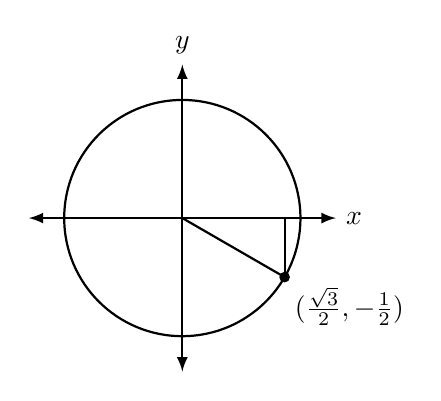
\begin{tikzpicture}[>=latex,scale=1.5,thick]
\draw [<->](-1.3,0)--(1.3,0) node [right] {$x$};
\draw [<->] (0,-1.3) -- (0,1.3) node [above] {$y$};
\draw (0,0) circle (1);
\draw [fill= black] (.866,-.5) circle (1pt);
	\draw (0,0) -- (.866,-.5) node [below right] {$(\frac{\sqrt{3}}{2}, -\frac{1}{2})$};
\draw (.866,-.5) -- (.866,0);
\end{tikzpicture}


%Image File Name: \texttt{\detokenize{fig03_05_ex_14}}\par
%TeX File Name: \texttt{\detokenize{fig_03_05_ex_14}}\par

%%%%%%%%%%%%%%%%%%%%%%%%

%\mysettikzname{fig03_05_ex_13}
%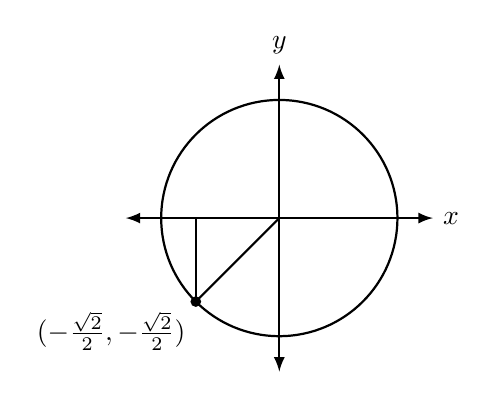
\begin{tikzpicture}[>=latex,scale=1.5,thick]
\draw [<->](-1.3,0)--(1.3,0) node [right] {$x$};
\draw [<->] (0,-1.3) -- (0,1.3) node [above] {$y$};
\draw (0,0) circle (1);
\draw [fill= black] (-.707,-.707) circle (1pt);
\draw (0,0) -- (-.707,-.707) node [below left] {$(-\frac{\sqrt{2}}{2}, -\frac{\sqrt{2}}{2})$};
\draw (-.707,-.707) -- (-.707,0);
\end{tikzpicture}



%Image File Name: \texttt{\detokenize{fig03_05_ex_13}}\par
%TeX File Name: \texttt{\detokenize{fig_03_05_ex_13}}\par

%%%%%%%%%%%%%%%%%%%%%%%%

%\mysettikzname{fig03_05_ex_12}
%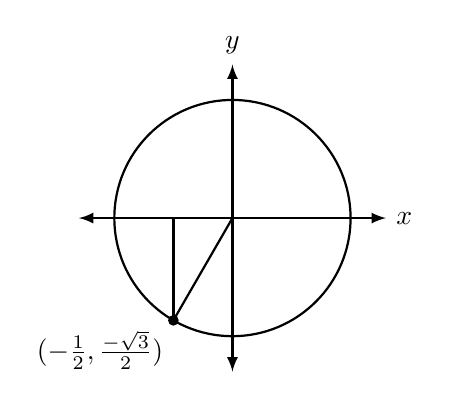
\begin{tikzpicture}[>=latex,scale=1.5,thick]
\draw [<->](-1.3,0)--(1.3,0) node [right] {$x$};
\draw [<->] (0,-1.3) -- (0,1.3) node [above] {$y$};
\draw (0,0) circle (1);
\draw [fill= black] (-.5,-.866) circle (1pt);
\draw (0,0) -- (-.5,-.866) node [below left] {$(-\frac{1}{2}, \frac{-\sqrt{3}}{2})$};
\draw (-.5,-.866) -- (-.5,0);
\end{tikzpicture}



%Image File Name: \texttt{\detokenize{fig03_05_ex_12}}\par
%TeX File Name: \texttt{\detokenize{fig_03_05_ex_12}}\par

%%%%%%%%%%%%%%%%%%%%%%%%

%\mysettikzname{fig03_04_ex_17}
%\input{fig_03_04_ex_17}

%Image File Name: \texttt{\detokenize{fig03_04_ex_17}}\par
%TeX File Name: \texttt{\detokenize{fig_03_04_ex_17}}\par

%%%%%%%%%%%%%%%%%%%%%%%%

%\mysettikzname{fig03_04_ex_16}
%\input{fig_03_04_ex_16}

%Image File Name: \texttt{\detokenize{fig03_04_ex_16}}\par
%TeX File Name: \texttt{\detokenize{fig_03_04_ex_16}}\par

%%%%%%%%%%%%%%%%%%%%%%%%

%\mysettikzname{figunitcircle}
%\input{fig_unitcircle}

%Image File Name: \texttt{\detokenize{figunitcircle}}\par
%TeX File Name: \texttt{\detokenize{fig_unitcircle}}\par

%%%%%%%%%%%%%%%%%%%%%%%%

%\mysettikzname{figineq_num_line7}
%\input{fig_ineq_num_line7}

%Image File Name: \texttt{\detokenize{figineq_num_line7}}\par
%TeX File Name: \texttt{\detokenize{fig_ineq_num_line7}}\par

%%%%%%%%%%%%%%%%%%%%%%%%

%\mysettikzname{figineq_num_line6}
%\input{fig_ineq_num_line6}

%Image File Name: \texttt{\detokenize{figineq_num_line6}}\par
%TeX File Name: \texttt{\detokenize{fig_ineq_num_line6}}\par

%%%%%%%%%%%%%%%%%%%%%%%%

%\mysettikzname{figineq_num_line5}
%\begin{tikzpicture}
	\draw[<->] (-4,0) -- (7,0);
	\draw (2,0.1) -- + (0,-0.2) node[below] {$2$};
	\draw (5,0.1) -- + (0,-0.2) node[below] {$5$};	
	\draw (-2,0.1) -- + (0,-0.2) node[below] {$-2$};
	\node at (-3,0.5) (a) {\ding{55}}; %xmark
	\node at (0,0.5) (a) {\ding{51}}; %checkmark
%	\node at (3,0.5) (a) {\ding{55}}; %xmark	
	\fill[white, draw=\colorone] (2,0) circle (0.6mm);
	\fill[white,draw=\colorone] (-2,0) circle (0.6mm);
	\fill[\colorone, draw=\colorone] (5,0) circle (0.6mm);	
\end{tikzpicture}
%\captionof{figure}{Graphically and numerically approximating $\lim_{x\to 3} \frac{x^2-x-6}{6x^2-19x+3}$ in Example \ref{ex_limit1}.}
%\caption{Graphically and numerically approximating $\lim_{x\to 3} \frac{x^2-x-6}{6x^2-19x+3}$ in Example \ref{ex_limit1}.}
%\label{fig:limit1}


%Image File Name: \texttt{\detokenize{figineq_num_line5}}\par
%TeX File Name: \texttt{\detokenize{fig_ineq_num_line5}}\par

%%%%%%%%%%%%%%%%%%%%%%%%

%\mysettikzname{figineq_num_line4}
%\input{fig_ineq_num_line4}

%Image File Name: \texttt{\detokenize{figineq_num_line4}}\par
%TeX File Name: \texttt{\detokenize{fig_ineq_num_line4}}\par

%%%%%%%%%%%%%%%%%%%%%%%%

%\mysettikzname{figineq_num_line3}
%\input{fig_ineq_num_line3}

%Image File Name: \texttt{\detokenize{figineq_num_line3}}\par
%TeX File Name: \texttt{\detokenize{fig_ineq_num_line3}}\par

%%%%%%%%%%%%%%%%%%%%%%%%

%\mysettikzname{figineq_num_line2}
%\begin{tikzpicture}
	\draw[<->] (0,0) -- (6,0);
	\draw (2,0.1) -- + (0,-0.2) node[below] {$2$};
	\draw (4,0.1) -- + (0,-0.2) node[below] {$4$};
	\node at (1,0.5) (a) {\ding{51}}; %checkmark
	\node at (5,0.5) (a) {\ding{51}}; %checkmark
	\node at (3,0.5) (a) {\ding{55}}; %xmark	
	\fill[white, draw=\colorone] (2,0) circle (0.6mm);
	\fill[white,draw=\colorone] (4,0) circle (0.6mm);
\end{tikzpicture}
%\captionof{figure}{Graphically and numerically approximating $\lim_{x\to 3} \frac{x^2-x-6}{6x^2-19x+3}$ in Example \ref{ex_limit1}.}
%\caption{Graphically and numerically approximating $\lim_{x\to 3} \frac{x^2-x-6}{6x^2-19x+3}$ in Example \ref{ex_limit1}.}
%\label{fig:limit1}


%Image File Name: \texttt{\detokenize{figineq_num_line2}}\par
%TeX File Name: \texttt{\detokenize{fig_ineq_num_line2}}\par

%%%%%%%%%%%%%%%%%%%%%%%%

%\mysettikzname{figineq_num_line1}
%\input{fig_ineq_num_line1}

%Image File Name: \texttt{\detokenize{figineq_num_line1}}\par
%TeX File Name: \texttt{\detokenize{fig_ineq_num_line1}}\par

%%%%%%%%%%%%%%%%%%%%%%%%

%\mysettikzname{fig02_04_ex_22}
%\begin{tikzpicture}
\begin{axis}[clip=false,width=\marginparwidth+25pt,tick label style={font=\scriptsize},minor x tick num=1,axis y line=middle,axis x line=middle,ymin=-1.1,ymax=3.1,extra y tick labels={},xmin=-1.1,xmax=4.1,name=myplot]
\addplot[domain=-1:4,smooth,variable=\x,\colorone] plot ({\x},{-0.66666*\x+2});
	\addplot[domain=-1:4, smooth, variable=\x,\colorone] plot({\x},{0});
	\addplot +[mark=none, \colorone] coordinates {(0, -1) (0, 3)};
	\fill[\colorone,draw=\colorone,thick] (axis cs:0,0) circle (1.5pt);
	\fill[\colorone,draw=\colorone,thick] (axis cs:0,2) circle (1.5pt);
	\fill[\colorone,draw=\colorone,thick] (axis cs:3,0) circle (1.5pt);
\end{axis}
\node [right] at (myplot.right of origin) {\scriptsize $x$};
\node [above] at (myplot.above origin) {\scriptsize $y$};
\end{tikzpicture}
%\captionof{figure}{Graphically and numerically approximating $\lim_{x\to 3} \frac{x^2-x-6}{6x^2-19x+3}$ in Example \ref{ex_limit1}.}
%\caption{Graphically and numerically approximating $\lim_{x\to 3} \frac{x^2-x-6}{6x^2-19x+3}$ in Example \ref{ex_limit1}.}
%\label{fig:limit1}


%Image File Name: \texttt{\detokenize{fig02_04_ex_22}}\par
%TeX File Name: \texttt{\detokenize{fig_02_04_ex_22}}\par

%%%%%%%%%%%%%%%%%%%%%%%%

%\mysettikzname{fig02_04_ex_21}
%\input{fig_02_04_ex_21}

%Image File Name: \texttt{\detokenize{fig02_04_ex_21}}\par
%TeX File Name: \texttt{\detokenize{fig_02_04_ex_21}}\par

%%%%%%%%%%%%%%%%%%%%%%%%

%\mysettikzname{fig02_04_ex_20}
%\input{fig_02_04_ex_20}

%Image File Name: \texttt{\detokenize{fig02_04_ex_20}}\par
%TeX File Name: \texttt{\detokenize{fig_02_04_ex_20}}\par

%%%%%%%%%%%%%%%%%%%%%%%%

%\mysettikzname{fig02_04_ex_19}
%\input{fig_02_04_ex_19}

%Image File Name: \texttt{\detokenize{fig02_04_ex_19}}\par
%TeX File Name: \texttt{\detokenize{fig_02_04_ex_19}}\par

%%%%%%%%%%%%%%%%%%%%%%%%

%\mysettikzname{fig02_02_ex_29}
%\input{fig_02_02_ex_29}

%Image File Name: \texttt{\detokenize{fig02_02_ex_29}}\par
%TeX File Name: \texttt{\detokenize{fig_02_02_ex_29}}\par

%%%%%%%%%%%%%%%%%%%%%%%%

%\mysettikzname{fig02_02_ex_28}
%\input{fig_02_02_ex_28}

%Image File Name: \texttt{\detokenize{fig02_02_ex_28}}\par
%TeX File Name: \texttt{\detokenize{fig_02_02_ex_28}}\par

%%%%%%%%%%%%%%%%%%%%%%%%

%\mysettikzname{fig02_02_ex_27}
%\begin{tikzpicture}
\begin{axis}[clip=false,width=\marginparwidth+25pt,tick label style={font=\scriptsize},minor x tick num=1,axis y line=middle,axis x line=middle,ymin=-5.1,ymax=5.1,extra y tick labels={},xmin=-6.1,xmax=1.1,name=myplot]
	\addplot[domain=-6:0,smooth,variable=\x,\colorone] plot ({\x},{-1*(\x+3)*(\x+3) +4});
\end{axis}
\node [right] at (myplot.right of origin) {\scriptsize $x$};
	\node [above] at (myplot.above origin) {\scriptsize $g(x)$};
\end{tikzpicture}
%\captionof{figure}{Graphically and numerically approximating $\lim_{x\to 3} \frac{x^2-x-6}{6x^2-19x+3}$ in Example \ref{ex_limit1}.}
%\caption{Graphically and numerically approximating $\lim_{x\to 3} \frac{x^2-x-6}{6x^2-19x+3}$ in Example \ref{ex_limit1}.}
%\label{fig:limit1}


%Image File Name: \texttt{\detokenize{fig02_02_ex_27}}\par
%TeX File Name: \texttt{\detokenize{fig_02_02_ex_27}}\par

%%%%%%%%%%%%%%%%%%%%%%%%

%\mysettikzname{fig02_02_ex_26}
%\input{fig_02_02_ex_26}

%Image File Name: \texttt{\detokenize{fig02_02_ex_26}}\par
%TeX File Name: \texttt{\detokenize{fig_02_02_ex_26}}\par

%%%%%%%%%%%%%%%%%%%%%%%%

%\mysettikzname{fig02_02_ex_25}
%\input{fig_02_02_ex_25}

%Image File Name: \texttt{\detokenize{fig02_02_ex_25}}\par
%TeX File Name: \texttt{\detokenize{fig_02_02_ex_25}}\par

%%%%%%%%%%%%%%%%%%%%%%%%

%\mysettikzname{fig02_02_ex_24}
%\input{fig_02_02_ex_24}

%Image File Name: \texttt{\detokenize{fig02_02_ex_24}}\par
%TeX File Name: \texttt{\detokenize{fig_02_02_ex_24}}\par

%%%%%%%%%%%%%%%%%%%%%%%%

%\mysettikzname{fig02_02_ex_23}
%\begin{tikzpicture}
\begin{axis}[clip=false,width=\marginparwidth+25pt,tick label style={font=\scriptsize},minor x tick num=1,axis y line=middle,axis x line=middle,ymin=-2.1,ymax=9.1,extra y tick labels={},xmin=-3.1,xmax=4.1,name=myplot]
	\addplot[domain=-2.77777:3.333333,smooth,variable=\x,\colorone] plot ({\x},{(\x-0.33333)*(\x-0.3333333) -0.11111111});
\end{axis}
\node [right] at (myplot.right of origin) {\scriptsize $q$};
	\node [above] at (myplot.above origin) {\scriptsize $p(q)$};
\end{tikzpicture}
%\captionof{figure}{Graphically and numerically approximating $\lim_{x\to 3} \frac{x^2-x-6}{6x^2-19x+3}$ in Example \ref{ex_limit1}.}
%\caption{Graphically and numerically approximating $\lim_{x\to 3} \frac{x^2-x-6}{6x^2-19x+3}$ in Example \ref{ex_limit1}.}
%\label{fig:limit1}


%Image File Name: \texttt{\detokenize{fig02_02_ex_23}}\par
%TeX File Name: \texttt{\detokenize{fig_02_02_ex_23}}\par

%%%%%%%%%%%%%%%%%%%%%%%%

\mysettikzname{fig02_02_ex_22}
\begin{tikzpicture}
\begin{axis}[clip=false,width=\marginparwidth+25pt,tick label style={font=\scriptsize},minor x tick num=1,axis y line=middle,axis x line=middle,ymin=-2.1,ymax=11.1,extra y tick labels={},xmin=-4.1,xmax=3.1,name=myplot]
	\addplot[domain=-4:2,smooth,variable=\x,\colorone] plot ({\x},{(\x+1)*(\x+1) + 2});
\end{axis}
\node [right] at (myplot.right of origin) {\scriptsize $t$};
	\node [above] at (myplot.above origin) {\scriptsize $f(t)$};
\end{tikzpicture}
%\captionof{figure}{Graphically and numerically approximating $\lim_{x\to 3} \frac{x^2-x-6}{6x^2-19x+3}$ in Example \ref{ex_limit1}.}
%\caption{Graphically and numerically approximating $\lim_{x\to 3} \frac{x^2-x-6}{6x^2-19x+3}$ in Example \ref{ex_limit1}.}
%\label{fig:limit1}


Image File Name: \texttt{\detokenize{fig02_02_ex_22}}\par
TeX File Name: \texttt{\detokenize{fig_02_02_ex_22}}\par

%%%%%%%%%%%%%%%%%%%%%%%%

%\mysettikzname{fig02_01_ex_28}
%\begin{tikzpicture}
\begin{axis}[clip=false,width=\marginparwidth+25pt,tick label style={font=\scriptsize},minor x tick num=1,axis y line=middle,axis x line=middle,ymin=-8.1,ymax=8.1,extra y tick labels={},xmin=-5.1,xmax=1.1,name=myplot]
	\addplot[domain=-4:0,smooth,variable=\x,\colorone] plot ({\x},{(\x+2)*(\x+2)*(\x+2)});
\end{axis}
\node [right] at (myplot.right of origin) {\scriptsize $x$};
\node [above] at (myplot.above origin) {\scriptsize $y$};
\end{tikzpicture}
%\captionof{figure}{Graphically and numerically approximating $\lim_{x\to 3} \frac{x^2-x-6}{6x^2-19x+3}$ in Example \ref{ex_limit1}.}
%\caption{Graphically and numerically approximating $\lim_{x\to 3} \frac{x^2-x-6}{6x^2-19x+3}$ in Example \ref{ex_limit1}.}
%\label{fig:limit1}


%Image File Name: \texttt{\detokenize{fig02_01_ex_28}}\par
%TeX File Name: \texttt{\detokenize{fig_02_01_ex_28}}\par

%%%%%%%%%%%%%%%%%%%%%%%%

%\mysettikzname{fig02_01_ex_30}
%\input{fig_02_01_ex_30}

%Image File Name: \texttt{\detokenize{fig02_01_ex_30}}\par
%TeX File Name: \texttt{\detokenize{fig_02_01_ex_30}}\par

%%%%%%%%%%%%%%%%%%%%%%%%

%\mysettikzname{fig02_01_ex_29}
%\input{fig_02_01_ex_29}

%Image File Name: \texttt{\detokenize{fig02_01_ex_29}}\par
%TeX File Name: \texttt{\detokenize{fig_02_01_ex_29}}\par

%%%%%%%%%%%%%%%%%%%%%%%%


%\mysettikzname{fig01_05_ex_23}
%\begin{tikzpicture}
\begin{axis}[clip=false,width=\marginparwidth+25pt,tick label style={font=\scriptsize},minor x tick num=1,axis y line=middle,axis x line=middle,ymin=-1.1,ymax=10.1,extra y tick labels={},xmin=-2.1,xmax=6.1,name=myplot]
	\addplot[domain=-2:6,smooth,variable=\x,\colorone] plot ({\x},{exp(-1*\x) + 1});
\end{axis}
\node [right] at (myplot.right of origin) {\scriptsize $x$};
\node [above] at (myplot.above origin) {\scriptsize $y$};
\end{tikzpicture}
%\captionof{figure}{Graphically and numerically approximating $\lim_{x\to 3} \frac{x^2-x-6}{6x^2-19x+3}$ in Example \ref{ex_limit1}.}
%\caption{Graphically and numerically approximating $\lim_{x\to 3} \frac{x^2-x-6}{6x^2-19x+3}$ in Example \ref{ex_limit1}.}
%\label{fig:limit1}


%Image File Name: \texttt{\detokenize{fig01_05_ex_23}}\par
%TeX File Name: \texttt{\detokenize{fig_01_05_ex_23}}\par

%%%%%%%%%%%%%%%%%%%%%%%%

%\mysettikzname{fig01_05_ex_22}
%\input{fig_01_05_ex_22}

%Image File Name: \texttt{\detokenize{fig01_05_ex_22}}\par
%TeX File Name: \texttt{\detokenize{fig_01_05_ex_22}}\par

%%%%%%%%%%%%%%%%%%%%%%%%

%\mysettikzname{fig01_05_ex_15}
%\begin{tikzpicture}
\begin{axis}[clip=false,width=\marginparwidth+25pt,tick label style={font=\scriptsize},minor x tick num=1,axis y line=middle,axis x line=middle,ymin=-1.1,ymax=6.1,extra y tick labels={},xmin=-4.1,xmax=4.1,name=myplot]
	\addplot[domain=-4:4,smooth,variable=\x,\colorone] plot ({\x},{0.66666*\x + 2.33333});
\end{axis}
\node [right] at (myplot.right of origin) {\scriptsize $x$};
\node [above] at (myplot.above origin) {\scriptsize $y$};
\end{tikzpicture}
%\captionof{figure}{Graphically and numerically approximating $\lim_{x\to 3} \frac{x^2-x-6}{6x^2-19x+3}$ in Example \ref{ex_limit1}.}
%\caption{Graphically and numerically approximating $\lim_{x\to 3} \frac{x^2-x-6}{6x^2-19x+3}$ in Example \ref{ex_limit1}.}
%\label{fig:limit1}


%Image File Name: \texttt{\detokenize{fig01_05_ex_15}}\par
%TeX File Name: \texttt{\detokenize{fig_01_05_ex_15}}\par

%%%%%%%%%%%%%%%%%%%%%%%%

%\mysettikzname{fig01_05_ex_14}
%\begin{tikzpicture}
\begin{axis}[clip=false,width=\marginparwidth+25pt,tick label style={font=\scriptsize},minor x tick num=1,axis y line=middle,axis x line=middle,ymin=-4.1,ymax=16.1,extra y tick labels={},xmin=-4.1,xmax=4.1,name=myplot]
	\addplot[domain=-4:-2,smooth,variable=\x,\colorone] plot ({\x},{\x*\x - 1});
	\addplot[domain=-2:4,smooth,variable=\x,\colorone] plot ({\x},{3*\x + 3});
	\fill[black,draw=black,thick] (axis cs:-2,3) circle (1.5pt);
	\fill[white,draw=black,thick] (axis cs:-2,-3) circle (1.5pt);
\end{axis}
\node [right] at (myplot.right of origin) {\scriptsize $t$};
\node [above] at (myplot.above origin) {\scriptsize $y$};
\end{tikzpicture}
%\captionof{figure}{Graphically and numerically approximating $\lim_{x\to 3} \frac{x^2-x-6}{6x^2-19x+3}$ in Example \ref{ex_limit1}.}
%\caption{Graphically and numerically approximating $\lim_{x\to 3} \frac{x^2-x-6}{6x^2-19x+3}$ in Example \ref{ex_limit1}.}
%\label{fig:limit1}


%Image File Name: \texttt{\detokenize{fig01_05_ex_14}}\par
%TeX File Name: \texttt{\detokenize{fig_01_05_ex_14}}\par

%%%%%%%%%%%%%%%%%%%%%%%%

%\mysettikzname{fig01_05_ex_13}
%\input{fig_01_05_ex_13}

%Image File Name: \texttt{\detokenize{fig01_05_ex_13}}\par
%TeX File Name: \texttt{\detokenize{fig_01_05_ex_13}}\par

%%%%%%%%%%%%%%%%%%%%%%%%

%\mysettikzname{fig01_05_ex_12}
%\input{fig_01_05_ex_12}

%Image File Name: \texttt{\detokenize{fig01_05_ex_12}}\par
%TeX File Name: \texttt{\detokenize{fig_01_05_ex_12}}\par

%%%%%%%%%%%%%%%%%%%%%%%%

%\mysettikzname{fig01_05_ex_11}
%\input{fig_01_05_ex_11}

%Image File Name: \texttt{\detokenize{fig01_05_ex_11}}\par
%TeX File Name: \texttt{\detokenize{fig_01_05_ex_11}}\par

%%%%%%%%%%%%%%%%%%%%%%%%

%\mysettikzname{fig01_05_ex_09}
%\input{fig_01_05_ex_09}

%Image File Name: \texttt{\detokenize{fig01_05_ex_09}}\par
%TeX File Name: \texttt{\detokenize{fig_01_05_ex_09}}\par

%%%%%%%%%%%%%%%%%%%%%%%%

%\mysettikzname{fig01_05_ex_10}
%\input{fig_01_05_ex_10}

%Image File Name: \texttt{\detokenize{fig01_05_ex_10}}\par
%TeX File Name: \texttt{\detokenize{fig_01_05_ex_10}}\par

%%%%%%%%%%%%%%%%%%%%%%%%

%\mysettikzname{fig01_05_ex_08}
%\begin{tikzpicture}
\begin{axis}[clip=false,width=\marginparwidth+25pt,tick label style={font=\scriptsize},minor x tick num=1,axis y line=middle,axis x line=middle,ymin=-1.1,ymax=9.1,extra y tick labels={},xmin=-3.1,xmax=3.1,name=myplot]
\addplot[domain=-3:0,smooth,variable=\x,\colorone] plot ({\x},{-1*\x*\x});
\fill[white,draw=black,thick] (axis cs:0,0) circle (1.5pt);
\addplot[domain=0:3,smooth,variable=\x,\colorone] plot ({\x},{(\x-1)*(\x-1)});
\fill[black,draw=black,thick] (axis cs:0,1) circle (1.5pt);
\fill[white,draw=black,thick] (axis cs:3,4) circle (1.5pt);
\end{axis}
\node [right] at (myplot.right of origin) {\scriptsize $x$};
\node [above] at (myplot.above origin) {\scriptsize $y$};
\end{tikzpicture}
%\captionof{figure}{Graphically and numerically approximating $\lim_{x\to 3} \frac{x^2-x-6}{6x^2-19x+3}$ in Example \ref{ex_limit1}.}
%\caption{Graphically and numerically approximating $\lim_{x\to 3} \frac{x^2-x-6}{6x^2-19x+3}$ in Example \ref{ex_limit1}.}
%\label{fig:limit1}


%Image File Name: \texttt{\detokenize{fig01_05_ex_08}}\par
%TeX File Name: \texttt{\detokenize{fig_01_05_ex_08}}\par

%%%%%%%%%%%%%%%%%%%%%%%%

%\mysettikzname{fig01_05_ex_07}
%\input{fig_01_05_ex_07}

%Image File Name: \texttt{\detokenize{fig01_05_ex_07}}\par
%TeX File Name: \texttt{\detokenize{fig_01_05_ex_07}}\par

%%%%%%%%%%%%%%%%%%%%%%%%

%\mysettikzname{fig01_05_ex_06}
%\input{fig_01_05_ex_06}

%Image File Name: \texttt{\detokenize{fig01_05_ex_06}}\par
%TeX File Name: \texttt{\detokenize{fig_01_05_ex_06}}\par

%%%%%%%%%%%%%%%%%%%%%%%%
2x
%\mysettikzname{figpiecewise2}
%\input{fig_piecewise2}

%Image File Name: \texttt{\detokenize{figpiecewise2}}\par
%TeX File Name: \texttt{\detokenize{fig_piecewise2}}\par

%%%%%%%%%%%%%%%%%%%%%%%%

%\mysettikzname{figpiecewise1}
%\input{fig_piecewise1}

%Image File Name: \texttt{\detokenize{figpiecewise1}}\par
%TeX File Name: \texttt{\detokenize{fig_piecewise1}}\par

%%%%%%%%%%%%%%%%%%%%%%%%

%\mysettikzname{figquadratic_transformation4}
%\input{fig_quadratic_transformation4}

%Image File Name: \texttt{\detokenize{figquadratic_transformation4}}\par
%TeX File Name: \texttt{\detokenize{fig_quadratic_transformation4}}\par

%%%%%%%%%%%%%%%%%%%%%%%%

%\mysettikzname{figquadratic_transformation3}
%\input{fig_quadratic_transformation3}

%Image File Name: \texttt{\detokenize{figquadratic_transformation3}}\par
%TeX File Name: \texttt{\detokenize{fig_quadratic_transformation3}}\par

%%%%%%%%%%%%%%%%%%%%%%%%

%\mysettikzname{figquadratic_transformation2}
%\input{fig_quadratic_transformation2}

%Image File Name: \texttt{\detokenize{figquadratic_transformation2}}\par
%TeX File Name: \texttt{\detokenize{fig_quadratic_transformation2}}\par

%%%%%%%%%%%%%%%%%%%%%%%%

%\mysettikzname{figquadratic_transformation1}
%\begin{tikzpicture}
\begin{axis}[clip=false,width=\marginparwidth+25pt,tick label style={font=\scriptsize},minor x tick num=1,axis y line=middle,axis x line=middle,ymin=-9.1,ymax=9.1,extra y tick labels={},xmin=-9.1,xmax=5=9.1,name=myplot]
	\addplot[domain=-3:3,smooth,variable=\x,\colorone, dotted] plot ({\x},{\x*\x});
	\addplot[domain=-5:1,smooth,variable=\x,\colortwo] plot ({\x},{(\x+2)*(\x+2)});
\end{axis}
\node [right] at (myplot.right of origin) {\scriptsize $x$};
\node [above] at (myplot.above origin) {\scriptsize $y$};
\end{tikzpicture}
%\captionof{figure}{Graphically and numerically approximating $\lim_{x\to 3} \frac{x^2-x-6}{6x^2-19x+3}$ in Example \ref{ex_limit1}.}
%\caption{Graphically and numerically approximating $\lim_{x\to 3} \frac{x^2-x-6}{6x^2-19x+3}$ in Example \ref{ex_limit1}.}
%\label{fig:limit1}


%Image File Name: \texttt{\detokenize{figquadratic_transformation1}}\par
%TeX File Name: \texttt{\detokenize{fig_quadratic_transformation1}}\par

%%%%%%%%%%%%%%%%%%%%%%%%

%\mysettikzname{figquadratic_shift_shrink}
%\begin{tikzpicture}
\begin{axis}[clip=false,width=\marginparwidth+25pt,tick label style={font=\scriptsize},minor x tick num=1,axis y line=middle,axis x line=middle,ymin=-2.1,ymax=9.1,extra y tick labels={},xmin=-3.1,xmax=3.1,name=myplot]
	\addplot[domain=-3:2,smooth,variable=\x,\colorone, dotted] plot ({\x},{(\x+1)*(\x+1)});
	\addplot[domain=-2:1,smooth,variable=\x,\colortwo] plot ({\x},{(2*\x+1)*(2*\x+1)});
	\fill[white,draw=black,thick] (axis cs:-0.5,0) circle (1.5pt);

\end{axis}
\node [right] at (myplot.right of origin) {\scriptsize $x$};
\node [above] at (myplot.above origin) {\scriptsize $y$};
\end{tikzpicture}
%\captionof{figure}{Graphically and numerically approximating $\lim_{x\to 3} \frac{x^2-x-6}{6x^2-19x+3}$ in Example \ref{ex_limit1}.}
%\caption{Graphically and numerically approximating $\lim_{x\to 3} \frac{x^2-x-6}{6x^2-19x+3}$ in Example \ref{ex_limit1}.}
%\label{fig:limit1}


%Image File Name: \texttt{\detokenize{figquadratic_shift_shrink}}\par
%TeX File Name: \texttt{\detokenize{fig_quadratic_shift_shrink}}\par

%%%%%%%%%%%%%%%%%%%%%%%%

%\mysettikzname{figquadratic_shift}
%\input{fig_quadratic_shift}

%Image File Name: \texttt{\detokenize{figquadratic_shift}}\par
%TeX File Name: \texttt{\detokenize{fig_quadratic_shift}}\par

%%%%%%%%%%%%%%%%%%%%%%%%

%\mysettikzname{fig2sine_shifted}
%\begin{tikzpicture}
\begin{axis}[clip=false,width=\marginparwidth+25pt,tick label style={font=\scriptsize},minor x tick num=1,axis y line=middle,axis x line=middle,ymin=-3.6,ymax=3.6,extra y tick labels={},xmin=-6.1,xmax=6.1,name=myplot, xtick={
        -4.7123889, -3.14159, -1.5708,
        1.5708, 3.14159, 4.7123889
    },
    xticklabels={
        $-\frac{3\pi}{2}$, $-\pi$, $-\frac{\pi}{2}$,
        $\frac{\pi}{2}$, $\pi$, $\frac{3\pi}{2}$
    }]
	\addplot[domain=-6:6,smooth,variable=\x,\colortwo] plot ({\x},{2*sin(deg(\x))-1});
\end{axis}
\node [right] at (myplot.right of origin) {\scriptsize $x$};
\node [above] at (myplot.above origin) {\scriptsize $y$};
\end{tikzpicture}
%\captionof{figure}{Graphically and numerically approximating $\lim_{x\to 3} \frac{x^2-x-6}{6x^2-19x+3}$ in Example \ref{ex_limit1}.}
%\caption{Graphically and numerically approximating $\lim_{x\to 3} \frac{x^2-x-6}{6x^2-19x+3}$ in Example \ref{ex_limit1}.}
%\label{fig:limit1}


%Image File Name: \texttt{\detokenize{fig2sine_shifted}}\par
%TeX File Name: \texttt{\detokenize{fig_2sine_shifted}}\par

%%%%%%%%%%%%%%%%%%%%%%%%

%\mysettikzname{fig2sine}
%\input{fig_2sine}

%Image File Name: \texttt{\detokenize{fig2sine}}\par
%TeX File Name: \texttt{\detokenize{fig_2sine}}\par

%%%%%%%%%%%%%%%%%%%%%%%%

%\mysettikzname{figvertical_flip}
%\input{fig_vertical_flip}

%Image File Name: \texttt{\detokenize{figvertical_flip}}\par
%TeX File Name: \texttt{\detokenize{fig_vertical_flip}}\par

%%%%%%%%%%%%%%%%%%%%%%%%

%\mysettikzname{figvertical_shrink}
%\begin{tikzpicture}
\begin{axis}[clip=false,width=\marginparwidth+25pt,tick label style={font=\scriptsize},minor x tick num=1,axis y line=middle,axis x line=middle,ymin=-8.1,ymax=8.1,extra y tick labels={},xmin=-3.1,xmax=3.1,name=myplot]
\addplot[domain=-2:2,smooth,variable=\x,\colorone, dotted] plot ({\x},{\x*\x*\x});
\addplot[domain=-2.52:2.52,smooth,variable=\x,\colortwo] plot ({\x},{0.5*\x*\x*\x});
\end{axis}
\node [right] at (myplot.right of origin) {\scriptsize $x$};
\node [above] at (myplot.above origin) {\scriptsize $y$};
\end{tikzpicture}
%\captionof{figure}{Graphically and numerically approximating $\lim_{x\to 3} \frac{x^2-x-6}{6x^2-19x+3}$ in Example \ref{ex_limit1}.}
%\caption{Graphically and numerically approximating $\lim_{x\to 3} \frac{x^2-x-6}{6x^2-19x+3}$ in Example \ref{ex_limit1}.}
%\label{fig:limit1}


%Image File Name: \texttt{\detokenize{figvertical_shrink}}\par
%TeX File Name: \texttt{\detokenize{fig_vertical_shrink}}\par

%%%%%%%%%%%%%%%%%%%%%%%%

%\mysettikzname{figvertical_shift}
%\input{fig_vertical_shift}

%Image File Name: \texttt{\detokenize{figvertical_shift}}\par
%TeX File Name: \texttt{\detokenize{fig_vertical_shift}}\par

%%%%%%%%%%%%%%%%%%%%%%%%

%\mysettikzname{figtangent_fnct}
%\begin{tikzpicture}
\begin{axis}[clip=false,width=\marginparwidth+25pt,tick label style={font=\scriptsize},minor x tick num=1,axis y line=middle,axis x line=middle,ymin=-10.6,ymax=10.6,extra y tick labels={},xmin=-6.1,xmax=6.1,name=myplot, xtick={
        -4.7123889, -3.14159, -1.5708,
        1.5708, 3.14159, 4.7123889
    },
    xticklabels={
        $-\frac{3\pi}{2}$, $-\pi$, $-\frac{\pi}{2}$,
        $\frac{\pi}{2}$, $\pi$, $\frac{3\pi}{2}$
    }]
	\addplot[domain=-6:-4.808,samples=400, smooth, variable=\x,\colorone] plot ({\x},{tan(deg(\x))});
	\addplot[domain=-4.618:-1.666,samples=400, variable=\x,\colorone] plot ({\x},{tan(deg(\x))});
	\addplot[domain=-1.4765:1.4753,samples=400, variable=\x,\colorone] plot ({\x},{tan(deg(\x))});
	\addplot[domain=1.666:4.618,samples=400, variable=\x,\colorone] plot ({\x},{tan(deg(\x))});
	\addplot[domain=4.806:6,samples=400, variable=\x,\colorone] plot ({\x},{tan(deg(\x))});
\end{axis}
\node [right] at (myplot.right of origin) {\scriptsize $x$};
\node [above] at (myplot.above origin) {\scriptsize $y$};
\end{tikzpicture}
%\captionof{figure}{Graphically and numerically approximating $\lim_{x\to 3} \frac{x^2-x-6}{6x^2-19x+3}$ in Example \ref{ex_limit1}.}
%\caption{Graphically and numerically approximating $\lim_{x\to 3} \frac{x^2-x-6}{6x^2-19x+3}$ in Example \ref{ex_limit1}.}
%\label{fig:limit1}


%Image File Name: \texttt{\detokenize{figtangent_fnct}}\par
%TeX File Name: \texttt{\detokenize{fig_tangent_fnct}}\par

%%%%%%%%%%%%%%%%%%%%%%%%

%\mysettikzname{figcosine}
%\input{fig_cosine}

%Image File Name: \texttt{\detokenize{figcosine}}\par
%TeX File Name: \texttt{\detokenize{fig_cosine}}\par

%%%%%%%%%%%%%%%%%%%%%%%%

%\mysettikzname{figsine}
%\input{fig_sine}

%Image File Name: \texttt{\detokenize{figsine}}\par
%TeX File Name: \texttt{\detokenize{fig_sine}}\par

%%%%%%%%%%%%%%%%%%%%%%%%

%\mysettikzname{figlog}
%\input{fig_log}

%Image File Name: \texttt{\detokenize{figlog}}\par
%TeX File Name: \texttt{\detokenize{fig_log}}\par

%%%%%%%%%%%%%%%%%%%%%%%%

%\mysettikzname{figexp}
%\input{fig_exp}

%Image File Name: \texttt{\detokenize{figexp}}\par
%TeX File Name: \texttt{\detokenize{fig_exp}}\par

%%%%%%%%%%%%%%%%%%%%%%%%

%\mysettikzname{figodd_poly}
%\input{fig_odd_poly}

%Image File Name: \texttt{\detokenize{figodd_poly}}\par
%TeX File Name: \texttt{\detokenize{fig_odd_poly}}\par

%%%%%%%%%%%%%%%%%%%%%%%%

%\mysettikzname{figeven_poly}
%\input{fig_even_poly}

%Image File Name: \texttt{\detokenize{figeven_poly}}\par
%TeX File Name: \texttt{\detokenize{fig_even_poly}}\par

%%%%%%%%%%%%%%%%%%%%%%%%	
	
%\mysettikzname{figcubic}
%\input{fig_cubic}

%Image File Name: \texttt{\detokenize{figcubic}}\par
%TeX File Name: \texttt{\detokenize{fig_cubic}}\par

%%%%%%%%%%%%%%%%%%%%%%%%
	
%\mysettikzname{figquadratic}
%\input{fig_quadratic}

%Image File Name: \texttt{\detokenize{figquadratic}}\par
%TeX File Name: \texttt{\detokenize{fig_quadratic}}\par

%%%%%%%%%%%%%%%%%%%%%%%%

%\mysettikzname{figplot_line_c}
%\begin{tikzpicture}
\begin{axis}[clip=false,width=\marginparwidth+25pt,tick label style={font=\scriptsize},minor x tick num=1,axis y line=middle,axis x line=middle,ymin=-4.1,ymax=5.1,extra y tick labels={},xmin=-3.1,xmax=3.1,name=myplot]
\fill[\colorone,draw={\colorone},thick] (axis cs:0,-3) circle (1.5pt);
\fill[\colorone,draw={\colorone},thick] (axis cs:1,-1) circle (1.5pt);
\addplot[domain=-0.5:3,smooth,variable=\x,\colorone] plot ({\x},{2*\x-3});
\end{axis}
\node [right] at (myplot.right of origin) {\scriptsize $x$};
\node [above] at (myplot.above origin) {\scriptsize $y$};
\end{tikzpicture}
%\captionof{figure}{Graphically and numerically approximating $\lim_{x\to 3} \frac{x^2-x-6}{6x^2-19x+3}$ in Example \ref{ex_limit1}.}
%\caption{Graphically and numerically approximating $\lim_{x\to 3} \frac{x^2-x-6}{6x^2-19x+3}$ in Example \ref{ex_limit1}.}
%\label{fig:limit1}


%Image File Name: \texttt{\detokenize{figplot_line_c}}\par
%TeX File Name: \texttt{\detokenize{fig_plot_line_c}}\par

%%%%%%%%%%%%%%%%%%%%%%%%

%\mysettikzname{figplot_line_b}
%\begin{tikzpicture}
\begin{axis}[clip=false,width=\marginparwidth+25pt,tick label style={font=\scriptsize},minor x tick num=1,axis y line=middle,axis x line=middle,ymin=-4.1,ymax=5.1,extra y tick labels={},xmin=-3.1,xmax=3.1,name=myplot]
\fill[\colorone,draw={\colorone},thick] (axis cs:0,-3) circle (1.5pt);
	\addplot [black,thick, dashed] coordinates {(0,-3) (1,-3) (1,-1)};
\fill[\colorone,draw={\colorone},thick] (axis cs:1,-1) circle (1.5pt);
\end{axis}
\node [right] at (myplot.right of origin) {\scriptsize $x$};
\node [above] at (myplot.above origin) {\scriptsize $y$};
\end{tikzpicture}
%\captionof{figure}{Graphically and numerically approximating $\lim_{x\to 3} \frac{x^2-x-6}{6x^2-19x+3}$ in Example \ref{ex_limit1}.}
%\caption{Graphically and numerically approximating $\lim_{x\to 3} \frac{x^2-x-6}{6x^2-19x+3}$ in Example \ref{ex_limit1}.}
%\label{fig:limit1}


%Image File Name: \texttt{\detokenize{figplot_line_b}}\par
%TeX File Name: \texttt{\detokenize{fig_plot_line_b}}\par

%%%%%%%%%%%%%%%%%%%%%%%%

%\mysettikzname{figplot_line_a}
%\input{fig_plot_line_a}

%Image File Name: \texttt{\detokenize{figplot_line_a}}\par
%TeX File Name: \texttt{\detokenize{fig_plot_line_a}}\par

%%%%%%%%%%%%%%%%%%%%%%%%	

%\mysettikzname{figline_x_int}
%\input{fig_x_int}

%Image File Name: \texttt{\detokenize{figline_x_int}}\par
%TeX File Name: \texttt{\detokenize{fig_line_x_int}}\par

%%%%%%%%%%%%%%%%%%%%%%%%	

%\mysettikzname{figline_y_int}
%\input{fig_line_y_int}

%Image File Name: \texttt{\detokenize{figline_y_int}}\par
%TeX File Name: \texttt{\detokenize{fig_line_y_int}}\par

%%%%%%%%%%%%%%%%%%%%%%%%	
	
%\mysettikzname{figperpend_lines}
%\input{fig_perpend_lines}

%Image File Name: \texttt{\detokenize{figperpend_lines}}\par
%TeX File Name: \texttt{\detokenize{fig_perpendlines}}\par

%%%%%%%%%%%%%%%%%%%%%%%%%	
	
%\mysettikzname{figparallel_lines}
%\input{fig_parallel_lines}

%Image File Name: \texttt{\detokenize{figparallel_lines}}\par
%TeX File Name: \texttt{\detokenize{fig_parallel_lines}}\par

%%%%%%%%%%%%%%%%%%%%%%%%%

%\mysettikzname{figline_zero_slope}
%\input{fig_line_zero_slope}

%Image File Name: \texttt{\detokenize{figline_zero_slope}}\par
%TeX File Name: \texttt{\detokenize{fig_line_zero_slope}}\par

%%%%%%%%%%%%%%%%%%%%%%%%%

%\mysettikzname{figline_neg_slope}
%\input{fig_line_neg_slope}

%Image File Name: \texttt{\detokenize{figline_neg_slope}}\par
%TeX File Name: \texttt{\detokenize{fig_line_neg_slope}}\par

%%%%%%%%%%%%%%%%%%%%%%%%%%

%\mysettikzname{figline_pos_slope}
%\input{fig_line_pos_slope}

%Image File Name: \texttt{\detokenize{figline_pos_slope}}\par
%TeX File Name: \texttt{\detokenize{fig_line_pos_slope}}\par

}% ends editmode check

\end{document}
